\section{Data}\label{Data}

\subsection{Introduction to Data}

The Euronext index methodology for OSEBX lays the foundation of data used in our analysis \parencite{OSEBX-rule-book}. Euronext collects data on OSEAX companies on CD, which are used to calculate upcoming index composition. The compositions are publicly announced on AD, and implemented on ED \parencite*{OSEBX-rule-book}, as shown in \autoref{fig:timeline-index-rebalancing}. For OSEBX, this timeline occurs twice a year, as the benchmark index rebalances semi-annually in March and September \parencite*{oslo-stock-exchange-news-web}. In \autoref{Results and discussion}, we use data from January 2006 to March 2023.

We decided to analyse three different prediction horizons so that for each index rebalancing event, we collect data from 30, 60, and 100 business days before ED. For example, for the index rebalancing event in March 2023, where ED is 2023-03-17, we collect data for all OSEAX companies in February of 2023, December and October of 2022. 

\begin{figure}[ht]
    \centering
    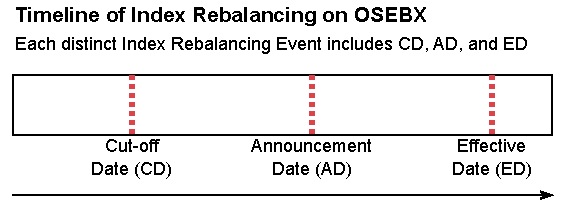
\includegraphics[width=0.8\linewidth]{images/timeline-cd-ad-ed.drawio (4).pdf}
    \vspace{1em}
    \caption{{OSEBX Index Rebalancing Timeline}}
    \subcaption*{Timeline of a single index rebalancing event on OSEBX with CD, AD, and ED. In the portfolio simulation in \autoref{Results and discussion} from 2010 to 2023 we experienced two distinct index rebalancing events each year (except 2020).}
    \label{fig:timeline-index-rebalancing}
\end{figure}

\subsection{Variables}

Euronext collects four key variables on CD reflecting the liquidity and size of companies \parencite{oslo-stock-exchange-news-web}. The first variable explains the proportion of a company's active trading days out of the total trading days in a given period \parencite*{OSEBX-rule-book}. We call this variable \texttt{trading\_status}. The second is turnover (electronic order book), which is the total value of shares traded at the end of the last 12 months up to and including CD, but excluding the 12 days with the highest turnover for each company \parencite*{OSEBX-rule-book}. We name this variable \texttt{turnover\_eob}. The next variable is the free float factor, which represents the free float market capitalisation for the total market value of shares that are publicly available for trading \parencite*{OSEBX-rule-book}. We call this variable \texttt{free\_float}. The last collected financial variable \texttt{icb\_supersector} is based on the industry classification benchmark (ICB) according to Dow Jones and FTSE \parencite{industry-classification-benchmark}. 

In short, Euronext collects the four variables above to calculate index composition, based on the publicly available index methodology \parencite{OSEBX-rule-book}. We do not review the rule book in greater detail here but in general the bigger \texttt{turnover\_eob}, \texttt{free\_float} and \texttt{trading\_status}, the more likely the company will be included on OSEBX according to \textcite{OSEBX-rule-book}. In this thesis, we seek to use the variables Euronext collects and use ML to predict upcoming index composition \textit{before} AD. If we can predict OSEBX changes before they are announced to the public, we may gain a temporal advantage. We seek to make our ML models as simple as possible, and therefore try not to use additional financial variables, which are not mentioned in the OSEBX rule book \parencite{OSEBX-rule-book}. We consider our findings to be easier to replicate and understand when not using any additional financial variables.


\subsubsection{Target Variable}

In our data, we introduce the binary target variable \texttt{index\_cp} to denote if a company is on the benchmark index OSEBX in the current period. This variable is equivalent to $Y_{i,t}$ explained in \autoref{Methodology}. The current period represents the time from the last ED to the upcoming ED. As such, we seek to predict \texttt{index\_cp} for the \textit{next} period. The binary target variable \texttt{index\_cp} is 1 if the company is on OSEBX, and 0 otherwise. Labeling our data set as such becomes an ML classification problem using SL \parencite{ban404-the-elements-of-statistical-learning}.

\subsubsection{Lag Variables}

 Certain selection criteria differ for companies being on/not on OSEBX \parencite{OSEBX-rule-book}. Furthermore, we are dependent on knowing the lagged target variable to use the conditional PPT, introduced in \autoref{Methodology}, where the lagged variable is denoted as $Y_{i, t-1}$. Therefore, we introduce lag variables showing the binary value for \texttt{index\_cp} in the previous periods. We introduce lag variables \texttt{index\_lag1}, \texttt{index\_lag2}, \texttt{index\_lag3}, and \texttt{index\_lag4} for the value of \texttt{index\_cp} in the previous 1 to 4 periods. Lag variables can be applied in R with the \texttt{stats::lag()} function \parencite{lag-variable-R}. 


\subsection{Data Sources}

We first collect the dates for relevant index rebalancing events from \textcite{oslo-stock-exchange-news-web}. Thereafter, we collect the benchmark index constituents on OSEAX and OSEBX the day after each ED, to make sure we know the index composition \textit{just after} each rebalancing event. Further, we collect the four financial variables for each company 30, 60, and 100 days in advance of the ED. This is done using a Bloomberg Terminal (BBG) \parencite{bloomberg-terminal}. For the portfolio simulation, we obtain stock prices for all companies using DataStream and a Refinitiv Terminal \parencite{nhh-data-stream}. Lastly, we obtain FF3 data by \textcite{bernt-fama-french}. 

We find public announcements on OSEBX constituents by \textcite{oslo-stock-exchange-news-web} dating back to 2002. In both the BBG and Refinitiv Terminals we are able to find variable and price data for some companies backdating to 2002, but also find significant missing values for other companies in the period before 2006. With this backdrop, we conclude to use data from January 2006 to March 2023, which after data manipulation yields a clean data set with no NA-values. The selected time horizon gives a total of two distinct index rebalancing events each year (except for 2020 when Euronext changed from rebalancing in June/December to March/September), all including a CD, AD, and ED, with the first and last ED being 2006-06-30 and 2023-03-17. All rebalancing dates (CD, AD, and ED for each rebalancing) are shown in \autoref{APPENDIX CD, AD, and ED from 2006 to 2023}.

\subsubsection{Bloomberg}

Specifically, we obtain data from BBG through the BBG Query Language (BQL) \parencite{bloomberg-professional-services-BQL}, implemented in Excel \parencite{BQL-fintools}. We retrieve historical data points through functions such as \texttt{BDH}, \texttt{BDP}, and \texttt{BQL} \parencite{dartmouth-BQL}. Please note that the specific BQL functions used are shown in \autoref{APPENDIX-Excel-Bloomberg-Add-In-BQL-Formulas}. In conclusion, after gathering data from BBG we were left with a data frame, including the following variables \texttt{DD} (the date the data was collected, 30, 60 or 100 days in advance of ED), \texttt{CD}, \texttt{AD}, \texttt{ED}, \texttt{ticker}, \texttt{name}, \texttt{icb\_supersector}, \texttt{free\_float}, \texttt{turnover\_eob},  \texttt{trading\_status} and \texttt{index\_cp}. Please note that \texttt{index\_cp} is defined as 1 if the observation's combination of ticker and ED exists in the data frame where only the OSEBX constituents are stored, which we also obtained from BBG. These variables are collected for each company listed on OSEAX since 2006.


\subsubsection{DataStream}
Because we want to simulate the historical performance of the constructed portfolios, we need to collect historical price data. In the simulations, we use volume-weighted average price (VWAP). The VWAP is a more accurate representation of the share price we could have bought or sold many stocks for, compared to the closing price (which is often reported when illustrating stock price development). VWAP is also commonly used to evaluate the performance of stock traders \parencite{madhavan-vwap}. The VWAP is collected using Refinitiv DataStream of all OSEAX companies in the period from 2006 to 2023 \parencite{nhh-data-stream}. Collecting these prices is done in practice through the Refinitiv terminal \parencite{lseg-refinitiv}, with an Excel add-in \parencite{refinitiv-excel-add-in}. The data frame generated by DataStream consists of one date column, and 487 columns representing each company to ever be listed on OSEAX since 2006. In conclusion, this data source gives us the historical VWAP for each company for each day since 2006.


\subsubsection{Fama-French 3-factor Model Data}

The FF3 factors on Oslo Stock Exchange (OSE), such as sensitivity to size $\beta_{i,SMB}$ and $\beta_{i,HML}$ is collected from a data file compiled by \textcite{bernt-fama-french}. Note that the collected FF3 is only available until 2022-05-31. As such, the actual portfolio simulation in \autoref{Results and discussion} goes until 2023-03-17, but the portfolio performance assessments use the period from 2010-02-28 to 2022-05-31 due to lack of FF3-factors after May of 2022.

\subsubsection{Risk-Free Interest Rate}

The risk-free interest rate $R_f$ is the expected return on a zero-risk investment, introduced by \textcite{irving-theory-of-interest}. It is useful when calculating the financial metrics discussed in \autoref{Theoretical background}. The risk-free rates $R_f$ in the Norwegian market are estimated and published by \textcite{bernt-risk-free}. We collect the monthly risk-free rate $R_f$ from \textcite{bernt-risk-free}, for the portfolio performance analysis period from 2010 to 2023. Thereafter we average these rates, which amounts to a monthly risk-free rate of $\approx$ 0.12\%, or 1.46\% annually. 

\subsection{Data Manipulation and Missing Data}
After obtaining the data presented, we still need to make certain operations to make it viable for analysis. We are now referring to the data set obtained from BBG, which ultimately is what will be used for our analysis. When a company is listed on OSEAX after the data cutoff point, we receive NA-values for those companies for the relevant period. This makes it somehow difficult to capture for our ML model if company data is not available at or before CD (or the date of prediction). Vice versa, it is difficult if a company is unlisted from OSEAX between CD and ED. We simply decide to remove rows where data on CD is not available, as this has minimal influence on our data set, and most of the companies entering OSEAX are not eligible for OSEBX the same period, with some exceptions, \parencite{OSEBX-rule-book}.

Regarding \texttt{icb\_supersector}, we are missing this variable for some companies before 2010. This stems from companies being classified before the standardisation toward ICB and then delisted. Luckily, we find the Global Industry Classification Standard (GICS) for these companies \parencite{global-industry-classification-standard}. Because ICB and GICS overlap, with 25 and 20 level 2 classifications each, we choose to manually estimate ICB for the relevant companies, as shown in \autoref{APPENDIX From GICS to ICB}. 

After cleaning the data sets for NA-values, we add the lagged variables \texttt{index\_lag1}, \texttt{index\_lag2}, \texttt{index\_lag3}, and \texttt{index\_lag4} using the \texttt{stats::lag()} function \parencite{lag-variable-R} in R. 

\subsection{Train-Test Split}

Splitting the data set into train and test data is an approach used in cross-validating ML models \parencite{geisser-cross-validation}. The idea of cross-validation is that the accuracy of the ML model is evaluated on a data set (test data), that is different than the data set it is trained on (train data). The approach is used to avoid over-fitting, as the test data set is not leaked to the train data set. To create a train-test split in our case, we use time series cross-validation (TSCV) \parencite{bergmeir-time-series-cross-validation}. Here we train the models on all historical rebalancing events before the point in time the predictions are made. Originally, we start by using train data up to before 2010, and thereafter add one period of train data for each new index rebalancing event. \autoref{fig:train-test-split} illustrates the split between the train and test data set we use in TSCV. As an example, when making predictions leading up to March of 2023 in \autoref{fig:train-test-split}, we train the ML model on all data up to that point. 

\begin{figure}[H]
    \centering
    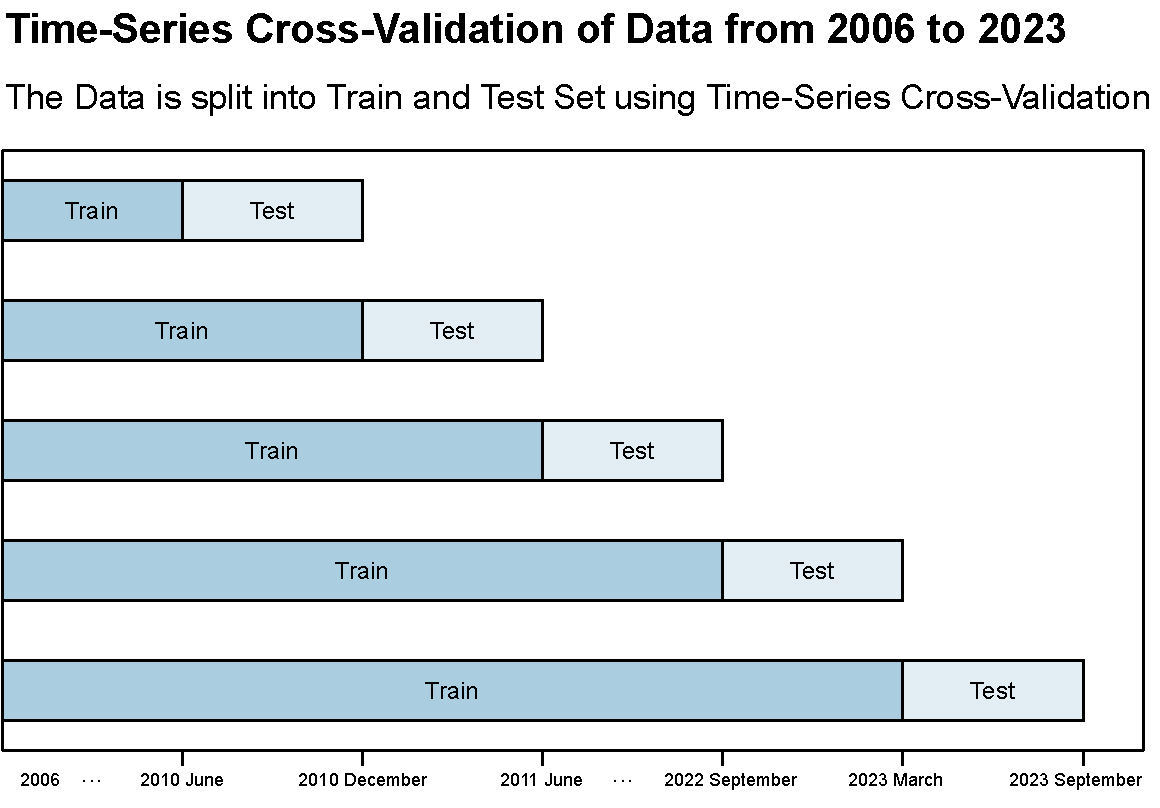
\includegraphics[width=0.8\textwidth]{images/train-test-split.drawio (4).pdf}
    \vspace{1em}
    \caption{{Time Series Cross-Validation}}
    \subcaption*{TSCV used in portfolio simulation for the trading strategy and enhanced index investing strategy.}
    \label{fig:train-test-split}
\end{figure}

\subsection{Summary of Data}

The final data set used in the ML models is summarised in \autoref{tab:final-data-set-predictor-target}. In short, we have generated three data sets containing these variables, one data set per prediction horizon of 30, 60, and 100 days before ED. As such, the \texttt{trading\_status}, \texttt{turnover\_eob} and \texttt{free\_float} will be somewhat different between the three data sets. The lagged variables from \texttt{index\_lag1} to \texttt{index\_lag4} will be the same across prediction horizons, as the time horizons of 30, 60, and 100 days do not overflow to the previous period. Note that \texttt{index\_cp} is the target variable, which after prediction indicates if the company will be or not be on OSEBX in the \textit{next} period. The lag variable \texttt{index\_lag1} indicates if a company is on OSEBX before the upcoming index rebalancing event. Also note that we use all the predictor variables in \autoref{tab:final-data-set-predictor-target} when predicting the target variable \texttt{index\_cp}. One could probably investigate further if all variables are necessary, and maybe even add other financial variables indicating size and liquidity. In short, we have chosen to keep the number of predictor variables relatively small compared to the amount of data points. The number of rows in the data sets is 5983, 5924, and 5891 for the 30, 60, and 100-day data frames respectively. The difference in the number of rows comes from the fast listings/delistings problem which means we need to discard more rows the longer the prediction horizon.



\begin{table}[H]
\centering
\begin{tabularx}{0.8\textwidth}{lXl}
\toprule
Variables & Explanation & Abbreviation \\ 
\midrule
{Informational variables:} \\
\texttt{data\_date}         & Data Date  & \texttt{DD} \\
\texttt{cutoff\_date}       & Cut-off Date  & \texttt{CD} \\
\texttt{announcement\_date} & Announcement Date & \texttt{AD} \\
\texttt{effective\_date}    & Effective Date & \texttt{ED} \\
\texttt{ticker}             & BBG Ticker \\
 & \\
{Predictor variables:} \\
\texttt{trading\_status}    & Share of Days Traded   & \texttt{TS}\\
\texttt{turnover\_eob}      & Turnover & \texttt{TO}\\
\texttt{icb\_supersector}   & ICB  & \texttt{ICB}\\
\texttt{free\_float}        & Free Float Market Cap & \texttt{FF} \\
\texttt{index\_lag1}        & \texttt{lag(index\_cp,1)} & \texttt{L1} \\
\texttt{index\_lag2}        & \texttt{lag(index\_cp,2)} & \texttt{L2} \\
\texttt{index\_lag3}        & \texttt{lag(index\_cp,3)} & \texttt{L3} \\
\texttt{index\_lag4}        & \texttt{lag(index\_cp,4)} & \texttt{L4} \\
 & \\
{Target variable:} \\
\texttt{index\_cp} & {1 if on OSEBX, 0 otherwise} &  \texttt{IC} \\
\bottomrule
\end{tabularx}
\vspace{1em}
\caption{{The Final Data Set of Predictor Variables and Target Variable}}
\subcaption*{Predictor Variables used in the ML models to predict the target variable \texttt{index\_cp} for the next period. Informational variables are from OSE Newsweb, financial predictor variables are from Euronext index methodology for OSEBX and lagged predictor variables are calculated.}
\label{tab:final-data-set-predictor-target}
\end{table}

Before we present our results, we briefly present a descriptive plot to better understand the data set. The number of listed companies on OSEAX and OSEBX is illustrated in \autoref{Members over time}, and we note that there are approximately 50$-$80 members on OSEBX for a given period, significantly less than those companies not included on OSEBX. There seem to be only about 5$-$10 additions and deletions in total for each period, as shown in \autoref{fig-OSEBX-Number-of-Additions-and-Deletions}.
\begin{figure}[H]
    \centering
    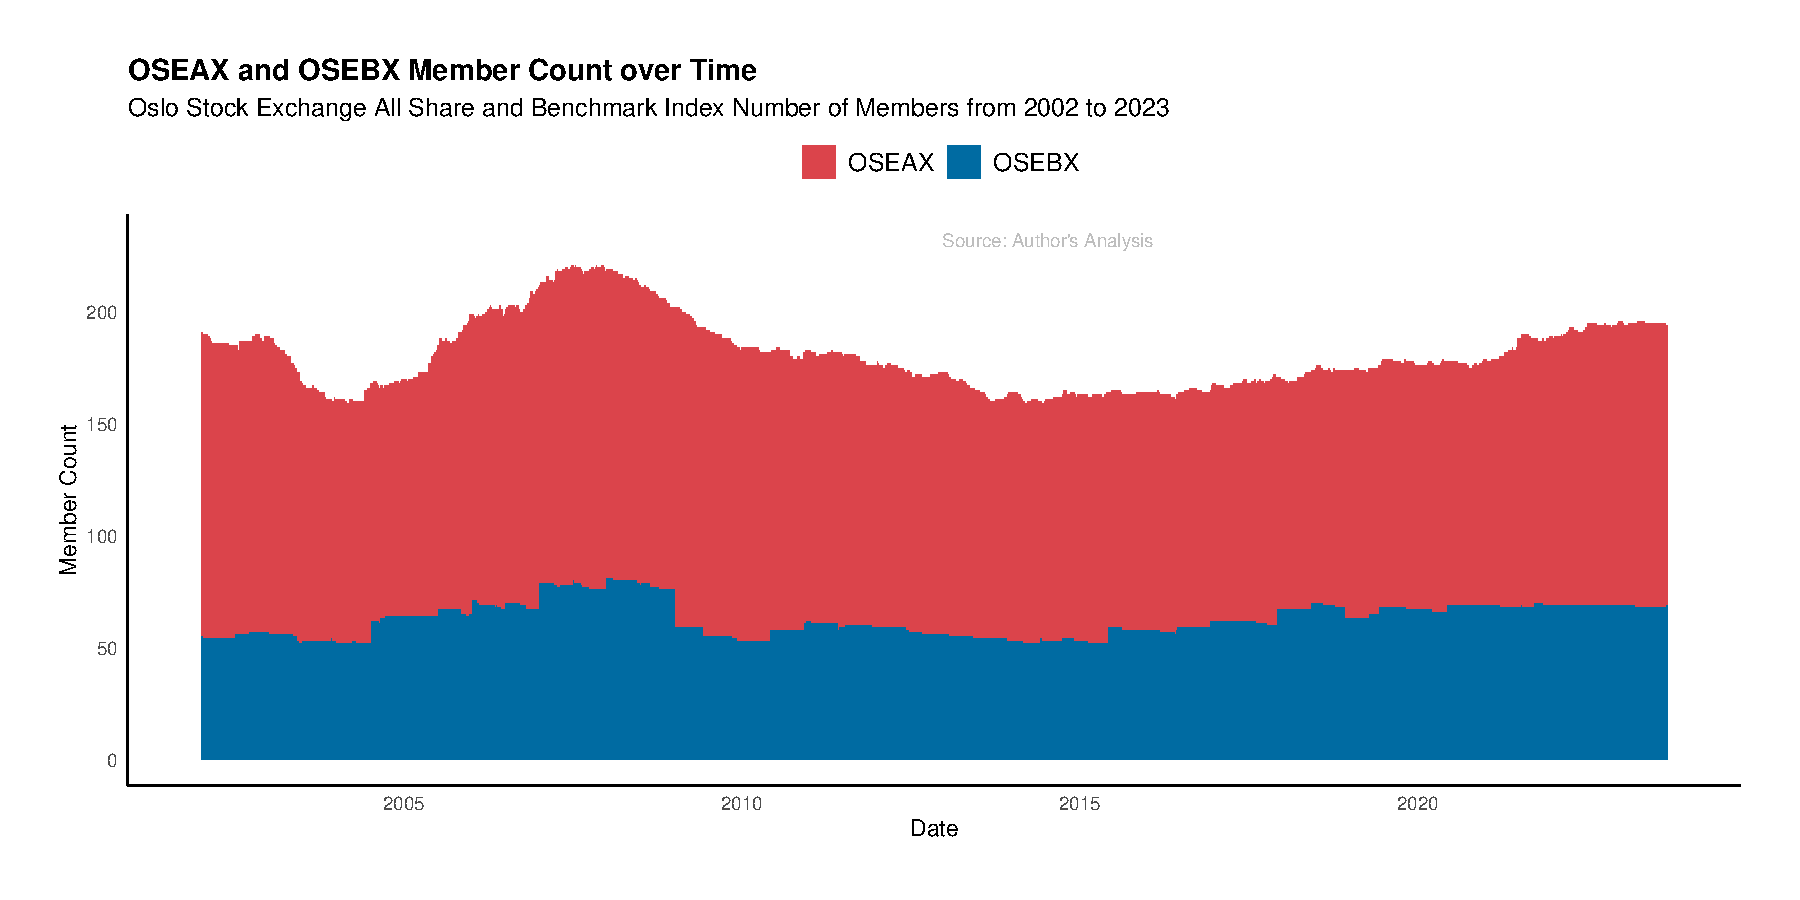
\includegraphics[width=\textwidth]{images/plotmemb_correct.pdf}
    \caption{{Members over Time}}
    \subcaption*{All OSEBX companies are also on OSEAX. Notice that OSEAX typically has about 200 companies, whereas 50-80 companies on OSEBX.}
    \label{Members over time}
\end{figure}









